\documentclass{article}

% content/resources/templates/preamble.tex
\usepackage[margin=0.6in]{geometry}
\author{Milav Dabgar}
\usepackage{amsmath,amssymb,amsthm}
\usepackage{booktabs}
\usepackage{multirow}
\usepackage{xcolor}
\usepackage{tcolorbox}
\tcbuselibrary{breakable,skins}
\usepackage[colorlinks=true,linkcolor=blue]{hyperref}
\usepackage{titlesec}
\usepackage{enumitem}
\usepackage{tikz}
\usepackage{pgfplots}
\usepackage{circuitikz}
\usepackage[version=4]{mhchem}
\usepackage{longtable}
\usepackage{array}
\usepackage{float}
\usepackage{caption}
\usepackage{listings}

\lstset{
  basicstyle=\small\ttfamily,
  breaklines=true,
  breakatwhitespace=false,
  postbreak=\mbox{\textcolor{red}{$\hookrightarrow$}\space},
  float=false,
  numbers=left,
  numberstyle=\tiny\color{gray},
  numbersep=10pt,
  xleftmargin=2em,
  keywordstyle=\color{blue},
  commentstyle=\color{green!60!black},
  stringstyle=\color{purple},
  backgroundcolor=\color{gray!5},
  showstringspaces=false,
  tabsize=2,
  captionpos=b,
  keepspaces=true,
  columns=flexible
}

\pgfplotsset{compat=1.18}
\usetikzlibrary{shapes,arrows,positioning,calc,patterns,decorations.pathmorphing,decorations.markings,arrows.meta}

% Color scheme
\definecolor{headcolor}{RGB}{0,102,204}
\definecolor{keycolor}{RGB}{220,20,60}
\definecolor{solutioncolor}{RGB}{34,139,34}
\definecolor{mnemoniccolor}{RGB}{148,0,211}
\definecolor{codecolor}{RGB}{0,0,100}

% Spacing
\setlength{\parskip}{3pt}
\setlist[itemize]{nosep}
\setlist[enumerate]{nosep}

% Title formatting
\titleformat{\section}{\Large\bfseries\color{headcolor}}{\thesection}{1em}{}
\titleformat{\subsection}{\large\bfseries\color{headcolor}}{\thesubsection}{1em}{}

% Pandoc tightlist compatibility
\providecommand{\tightlist}{%
  \setlength{\itemsep}{0pt}\setlength{\parskip}{0pt}}

% Pandoc longtable compatibility
\newcounter{none}
\def\thenone{}


% content/resources/templates/english-boxes.tex

% Custom environments
\newtcolorbox{solutionbox}{
 breakable,
 enhanced,
 colback=solutioncolor!5!white,
 colframe=solutioncolor!75!black,
 fonttitle=\bfseries,
 title=Solution
}

\newtcolorbox{solutionboxnobreak}{
 colback=solutioncolor!5!white,
 colframe=solutioncolor!75!black,
 fonttitle=\bfseries,
 title=Solution
}

\newtcolorbox{keyformula}{
 breakable,
 enhanced,
 colback=keycolor!5!white,
 colframe=keycolor!75!black,
 fonttitle=\bfseries,
 title=Key Formula
}

\newtcolorbox{mnemonicboxenv}{
 breakable,
 enhanced,
 colback=mnemoniccolor!5!white,
 colframe=mnemoniccolor!75!black,
 fonttitle=\bfseries,
 title=Mnemonic
}

\newcommand{\mnemonicbox}[1]{%
  \begin{mnemonicboxenv}
    #1
  \end{mnemonicboxenv}
}


% Custom commands for GTU solutions
% This file defines semantic commands for consistent formatting

% Question command with automatic formatting
\newcommand{\question}[2]{%
  \section*{Question #1}%
  \textbf{#2}%
}

% OR question variant
\newcommand{\questionor}[2]{%
  \section*{Question #1 OR}%
  \textbf{#2}%
}

% Proper table environment with caption
\newenvironment{answertable}[1]{%
  \begin{table}[htbp]
  \centering
  \caption{#1}
}{%
  \end{table}
}

% Proper figure environment for diagrams
\newenvironment{answerdiagram}[1]{%
  \begin{figure}[htbp]
  \centering
  \caption{#1}
}{%
  \end{figure}
}

% Semantic markup for key terms
\newcommand{\keyword}[1]{\textbf{#1}}
\newcommand{\code}[1]{\texttt{#1}}
\newcommand{\classname}[1]{\texttt{#1}}
\newcommand{\methodname}[1]{\texttt{#1}}

% Proper quotation marks
\newcommand{\mnemonic}[1]{``#1''}


\title{Mathematics-I (DI01000021) - Winter 2024 Solution}
\date{January 2, 2025}

\begin{document}
\maketitle

\questionmarks{Q.1}{14}{Fill in the blanks/MCQs using appropriate choice from the given options.}

\questionmarks{Q1.1}{1}{$\begin{vmatrix} 5 & 1 \\ 2 & 3 \end{vmatrix} = $ \_\_\_\_\_\_\_}
\begin{solutionbox}
\textbf{Answer}: b. 13

\textbf{Solution}:
For 2×2 determinant $\begin{vmatrix} a & b \\ c & d \end{vmatrix} = ad - bc$

$\begin{vmatrix} 5 & 1 \\ 2 & 3 \end{vmatrix} = (5 \times 3) - (1 \times 2) = 15 - 2 = 13$
\end{solutionbox}

\questionmarks{Q1.2}{1}{If $\begin{vmatrix} x & 1 \\ 2 & 1 \end{vmatrix} = 0$ then $x = $ \_\_\_\_\_\_\_}
\begin{solutionbox}
\textbf{Answer}: b. 2

\textbf{Solution}:
$\begin{vmatrix} x & 1 \\ 2 & 1 \end{vmatrix} = x \times 1 - 1 \times 2 = x - 2 = 0$

Therefore, $x = 2$
\end{solutionbox}

\questionmarks{Q1.3}{1}{If $f(x) = x^2$ then $f(-1) = $ \_\_\_\_\_\_\_}
\begin{solutionbox}
\textbf{Answer}: a. 1

\textbf{Solution}:
$f(x) = x^2$
$f(-1) = (-1)^2 = 1$
\end{solutionbox}

\questionmarks{Q1.4}{1}{$\log_{10} 1 = $ \_\_\_\_\_\_\_}
\begin{solutionbox}
\textbf{Answer}: b. 0

\textbf{Solution}:
By logarithm property: $\log_a 1 = 0$ for any base $a > 0$
Therefore, $\log_{10} 1 = 0$
\end{solutionbox}

\questionmarks{Q1.5}{1}{$\sin \frac{\pi}{2} + \cos \frac{\pi}{2} = $ \_\_\_\_\_\_\_}
\begin{solutionbox}
\textbf{Answer}: c. 1

\textbf{Solution}:
$\sin \frac{\pi}{2} = 1$ and $\cos \frac{\pi}{2} = 0$
Therefore, $\sin \frac{\pi}{2} + \cos \frac{\pi}{2} = 1 + 0 = 1$
\end{solutionbox}

\questionmarks{Q1.6}{1}{$\tan^{-1}(1) = $ \_\_\_\_\_\_\_}
\begin{solutionbox}
\textbf{Answer}: a. $\frac{\pi}{4}$

\textbf{Solution}:
$\tan \frac{\pi}{4} = 1$
Therefore, $\tan^{-1}(1) = \frac{\pi}{4}$
\end{solutionbox}

\questionmarks{Q1.7}{1}{$\frac{2\pi}{3}$ radian = \_\_\_\_\_\_\_ degree}
\begin{solutionbox}
\textbf{Answer}: d. 120

\textbf{Solution}:
To convert radians to degrees: $\text{degrees} = \text{radians} \times \frac{180}{\pi}$
$\frac{2\pi}{3} \times \frac{180}{\pi} = \frac{2 \times 180}{3} = \frac{360}{3} = 120\textdegree$
\end{solutionbox}

\questionmarks{Q1.8}{1}{$\hat{i} \times \hat{j} = $ \_\_\_\_\_\_\_}
\begin{solutionbox}
\textbf{Answer}: c. $\hat{k}$

\textbf{Solution}:
By right-hand rule for cross product:
$\hat{i} \times \hat{j} = \hat{k}$
\end{solutionbox}

\questionmarks{Q1.9}{1}{$|\hat{i} + \hat{j} + \hat{k}| = $ \_\_\_\_\_\_\_}
\begin{solutionbox}
\textbf{Answer}: d. $\sqrt{3}$

\textbf{Solution}:
$|\hat{i} + \hat{j} + \hat{k}| = \sqrt{1^2 + 1^2 + 1^2} = \sqrt{3}$
\end{solutionbox}

\questionmarks{Q1.10}{1}{Slope of line $2x + y - 3 = 0$ is \_\_\_\_\_\_\_}
\begin{solutionbox}
\textbf{Answer}: a. -2

\textbf{Solution}:
Convert to slope-intercept form: $y = -2x + 3$
Slope = coefficient of $x = -2$
\end{solutionbox}

\questionmarks{Q1.11}{1}{Radius of circle $x^2 + y^2 = 81$ is \_\_\_\_\_\_\_}
\begin{solutionbox}
\textbf{Answer}: b. 9

\textbf{Solution}:
Standard form: $x^2 + y^2 = r^2$
Here, $r^2 = 81$, so $r = 9$
\end{solutionbox}

\questionmarks{Q1.12}{1}{$\lim\limits_{n \to \infty} \frac{1}{n} = $ \_\_\_\_\_\_\_}
\begin{solutionbox}
\textbf{Answer}: c. 0

\textbf{Solution}:
As $n$ approaches infinity, $\frac{1}{n}$ approaches 0
\end{solutionbox}

\questionmarks{Q1.13}{1}{$\lim\limits_{x \to 1} (x^2 + x + 1) = $ \_\_\_\_\_\_\_}
\begin{solutionbox}
\textbf{Answer}: a. 3

\textbf{Solution}:
Direct substitution: $(1)^2 + (1) + 1 = 1 + 1 + 1 = 3$
\end{solutionbox}

\questionmarks{Q1.14}{1}{$\lim\limits_{\theta \to 0} \frac{\tan \theta}{\theta} = $ \_\_\_\_\_\_\_}
\begin{solutionbox}
\textbf{Answer}: b. 1

\textbf{Solution}:
This is a standard limit: $\lim\limits_{\theta \to 0} \frac{\tan \theta}{\theta} = 1$
\end{solutionbox}

\questionmarks{Q.2 (A)}{6}{Attempt any two}

\questionmarks{Q2.1}{3}{Find the value of $\begin{vmatrix} 1 & 3 & 1 \\ 2 & -1 & 0 \\ 4 & -2 & 5 \end{vmatrix}$}
\begin{solutionbox}
\textbf{Answer}:

\textbf{Solution}:
Using expansion along second row (has zero):
$= -2\begin{vmatrix} 3 & 1 \\ -2 & 5 \end{vmatrix} + (-1)\begin{vmatrix} 1 & 1 \\ 4 & 5 \end{vmatrix} + 0$

$= -2(15 + 2) - 1(5 - 4)$
$= -2(17) - 1(1)$
$= -34 - 1 = -35$

\begin{center}
\captionof{table}{Determinant Calculation Steps}
\begin{tabulary}{\linewidth}{|L|L|L|}
\hline
\textbf{Step} & \textbf{Calculation} & \textbf{Result} \\ \hline
Minor 1 & $(3 \times 5) - (1 \times -2)$ & 17 \\ \hline
Minor 2 & $(1 \times 5) - (1 \times 4)$ & 1 \\ \hline
Final & $-2(17) - 1(1)$ & -35 \\ \hline
\end{tabulary}
\end{center}
\end{solutionbox}

\questionmarks{Q2.2}{3}{If $f(x) = x^3 + 5$ then find $f(0)$, $f(1)$ and $f(-1)$}
\begin{solutionbox}
\textbf{Answer}:

\textbf{Solution}:
Given: $f(x) = x^3 + 5$

$f(0) = (0)^3 + 5 = 0 + 5 = 5$
$f(1) = (1)^3 + 5 = 1 + 5 = 6$
$f(-1) = (-1)^3 + 5 = -1 + 5 = 4$

\begin{center}
\captionof{table}{Function Values}
\begin{tabulary}{\linewidth}{|L|L|L|}
\hline
\textbf{Input} & \textbf{Calculation} & \textbf{Output} \\ \hline
$f(0)$ & $0^3 + 5$ & 5 \\ \hline
$f(1)$ & $1^3 + 5$ & 6 \\ \hline
$f(-1)$ & $(-1)^3 + 5$ & 4 \\ \hline
\end{tabulary}
\end{center}
\end{solutionbox}

\questionmarks{Q2.3}{3}{Prove that $\tan^{-1}\left(\frac{1}{2}\right) + \tan^{-1}\left(\frac{1}{3}\right) = \frac{\pi}{4}$}
\begin{solutionbox}
\textbf{Answer}:

\textbf{Solution}:
Using formula: $\tan^{-1}a + \tan^{-1}b = \tan^{-1}\left(\frac{a+b}{1-ab}\right)$

Let $a = \frac{1}{2}$, $b = \frac{1}{3}$

$\tan^{-1}\left(\frac{1}{2}\right) + \tan^{-1}\left(\frac{1}{3}\right) = \tan^{-1}\left(\frac{\frac{1}{2} + \frac{1}{3}}{1 - \frac{1}{2} \times \frac{1}{3}}\right)$

$= \tan^{-1}\left(\frac{\frac{5}{6}}{1 - \frac{1}{6}}\right) = \tan^{-1}\left(\frac{\frac{5}{6}}{\frac{5}{6}}\right) = \tan^{-1}(1) = \frac{\pi}{4}$

Hence proved.
\end{solutionbox}

\questionmarks{Q.2 (B)}{8}{Attempt any two}

\questionmarks{Q2.1}{4}{If $f(x) = \frac{x-1}{x+1}$ then prove that $f(x) \cdot f(-x) = 1$}
\begin{solutionbox}
\textbf{Answer}:

\textbf{Solution}:
Given: $f(x) = \frac{x-1}{x+1}$

First find $f(-x)$:
$f(-x) = \frac{(-x)-1}{(-x)+1} = \frac{-x-1}{-x+1} = \frac{-(x+1)}{-(x-1)} = \frac{x+1}{x-1}$

Now calculate $f(x) \cdot f(-x)$:
$f(x) \cdot f(-x) = \frac{x-1}{x+1} \cdot \frac{x+1}{x-1} = \frac{(x-1)(x+1)}{(x+1)(x-1)} = 1$

Hence proved.
\end{solutionbox}

\questionmarks{Q2.2}{4}{If $\log\left(\frac{x+y}{2}\right) = \frac{1}{2}(\log x + \log y)$ then prove that $x = y$}
\begin{solutionbox}
\textbf{Answer}:

\textbf{Solution}:
Given: $\log\left(\frac{x+y}{2}\right) = \frac{1}{2}(\log x + \log y)$

Using logarithm properties:
$\frac{1}{2}(\log x + \log y) = \frac{1}{2}\log(xy) = \log\sqrt{xy}$

So: $\log\left(\frac{x+y}{2}\right) = \log\sqrt{xy}$

Taking antilog: $\frac{x+y}{2} = \sqrt{xy}$

Squaring both sides: $\left(\frac{x+y}{2}\right)^2 = xy$

$\frac{(x+y)^2}{4} = xy$

$(x+y)^2 = 4xy$

$x^2 + 2xy + y^2 = 4xy$

$x^2 - 2xy + y^2 = 0$

$(x-y)^2 = 0$

Therefore, $x = y$. Hence proved.
\end{solutionbox}

\questionmarks{Q2.3}{4}{Solve $\log(x+3) + \log(x-3) = \log 27$}
\begin{solutionbox}
\textbf{Answer}:

\textbf{Solution}:
Given: $\log(x+3) + \log(x-3) = \log 27$

Using logarithm property: $\log a + \log b = \log(ab)$
$\log[(x+3)(x-3)] = \log 27$

Taking antilog: $(x+3)(x-3) = 27$

$x^2 - 9 = 27$

$x^2 = 36$

$x = \pm 6$

\textbf{Check validity:}

\begin{itemize}
\item For $x = 6$: $x+3 = 9 > 0$ and $x-3 = 3 > 0$ ✓
\item For $x = -6$: $x+3 = -3 < 0$ (invalid for logarithm)
\end{itemize}

Therefore, $x = 6$
\end{solutionbox}

\questionmarks{Q.3 (A)}{6}{Attempt any two}

\questionmarks{Q3.1}{3}{Prove that $\frac{\sin\left(\frac{\pi}{2}+\theta\right)}{\cos(\pi-\theta)} + \frac{\tan(\pi-\theta)}{\cot\left(\frac{3\pi}{2}-\theta\right)} + \frac{\text{cosec}\left(\frac{\pi}{2}-\theta\right)}{\sec(\pi+\theta)} = -3$}
\begin{solutionbox}
\textbf{Answer}:

\textbf{Solution}:
Using trigonometric identities:

$\sin\left(\frac{\pi}{2}+\theta\right) = \cos\theta$
$\cos(\pi-\theta) = -\cos\theta$
$\tan(\pi-\theta) = -\tan\theta$
$\cot\left(\frac{3\pi}{2}-\theta\right) = \tan\theta$
$\text{cosec}\left(\frac{\pi}{2}-\theta\right) = \sec\theta$
$\sec(\pi+\theta) = -\sec\theta$

Substituting:
$\frac{\cos\theta}{-\cos\theta} + \frac{-\tan\theta}{\tan\theta} + \frac{\sec\theta}{-\sec\theta}$

$= -1 + (-1) + (-1) = -3$

Hence proved.
\end{solutionbox}

\questionmarks{Q3.2}{3}{Prove that $\tan 55\textdegree = \frac{\cos 10\textdegree + \sin 10\textdegree}{\cos 10\textdegree - \sin 10\textdegree}$}
\begin{solutionbox}
\textbf{Answer}:

\textbf{Solution}:
We know that $\tan 55\textdegree = \tan(45\textdegree + 10\textdegree)$

Using formula: $\tan(A + B) = \frac{\tan A + \tan B}{1 - \tan A \tan B}$

$\tan 55\textdegree = \frac{\tan 45\textdegree + \tan 10\textdegree}{1 - \tan 45\textdegree \tan 10\textdegree} = \frac{1 + \tan 10\textdegree}{1 - \tan 10\textdegree}$

Now, $\tan 10\textdegree = \frac{\sin 10\textdegree}{\cos 10\textdegree}$

$\tan 55\textdegree = \frac{1 + \frac{\sin 10\textdegree}{\cos 10\textdegree}}{1 - \frac{\sin 10\textdegree}{\cos 10\textdegree}} = \frac{\cos 10\textdegree + \sin 10\textdegree}{\cos 10\textdegree - \sin 10\textdegree}$

Hence proved.
\end{solutionbox}

\questionmarks{Q3.3}{3}{If $\vec{a} = 2\hat{i} + 3\hat{j} + \hat{k}$, $\vec{b} = \hat{i} + \hat{j} + \hat{k}$ and $\vec{c} = 3\hat{i} + \hat{j} + \hat{k}$ then find $2\vec{a} + \vec{b} - \vec{c}$}
\begin{solutionbox}
\textbf{Answer}:

\textbf{Solution}:
Given:
$\vec{a} = 2\hat{i} + 3\hat{j} + \hat{k}$
$\vec{b} = \hat{i} + \hat{j} + \hat{k}$
$\vec{c} = 3\hat{i} + \hat{j} + \hat{k}$

$2\vec{a} = 2(2\hat{i} + 3\hat{j} + \hat{k}) = 4\hat{i} + 6\hat{j} + 2\hat{k}$

$2\vec{a} + \vec{b} - \vec{c} = (4\hat{i} + 6\hat{j} + 2\hat{k}) + (\hat{i} + \hat{j} + \hat{k}) - (3\hat{i} + \hat{j} + \hat{k})$

$= (4 + 1 - 3)\hat{i} + (6 + 1 - 1)\hat{j} + (2 + 1 - 1)\hat{k}$

$= 2\hat{i} + 6\hat{j} + 2\hat{k}$
\end{solutionbox}

\questionmarks{Q.3 (B)}{8}{Attempt any two}

\questionmarks{Q3.1}{4}{Prove that $\frac{\sin(x-y)}{\cos x \cos y} + \frac{\sin(y-z)}{\cos y \cos z} + \frac{\sin(z-x)}{\cos z \cos x} = 0$}
\begin{solutionbox}
\textbf{Answer}:

\textbf{Solution}:
Using identity: $\sin(A-B) = \sin A \cos B - \cos A \sin B$

$\frac{\sin(x-y)}{\cos x \cos y} = \frac{\sin x \cos y - \cos x \sin y}{\cos x \cos y} = \tan x - \tan y$

Similarly:
$\frac{\sin(y-z)}{\cos y \cos z} = \tan y - \tan z$
$\frac{\sin(z-x)}{\cos z \cos x} = \tan z - \tan x$

Adding all three:
$(\tan x - \tan y) + (\tan y - \tan z) + (\tan z - \tan x) = 0$

Hence proved.
\end{solutionbox}

\questionmarks{Q3.2}{4}{Draw graph of $y = \cos x$ for $0 \leq x \leq \pi$}
\begin{solutionbox}
\textbf{Answer}:

\textbf{Solution}:

\begin{figure}[h]
\centering
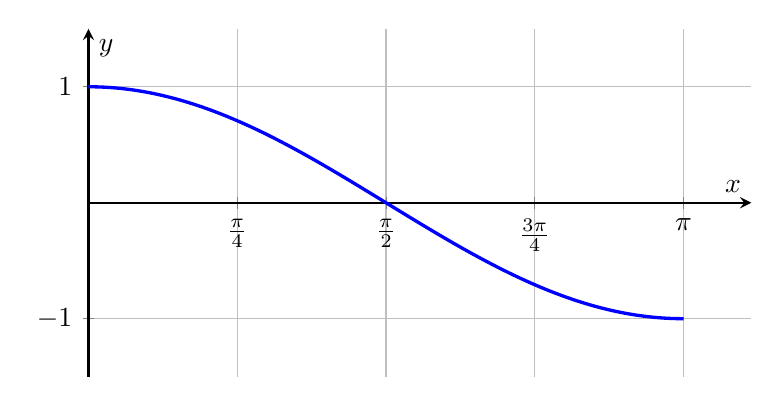
\begin{tikzpicture}
\begin{axis}[
    width=10cm,
    height=6cm,
    axis lines=center,
    xlabel={$x$},
    ylabel={$y$},
    xmin=0, xmax=3.5,
    ymin=-1.5, ymax=1.5,
    xtick={0, 0.785, 1.571, 2.356, 3.142},
    xticklabels={$0$, $\frac{\pi}{4}$, $\frac{\pi}{2}$, $\frac{3\pi}{4}$, $\pi$},
    ytick={-1, 0, 1},
    grid=major,
    samples=100,
    domain=0:3.142,
    smooth,
    thick
]
    \addplot[color=blue, very thick] {cos(deg(x))};
\end{axis}
\end{tikzpicture}
\caption{Graph of $y = \cos x$ for $0 \leq x \leq \pi$}
\end{figure}

\captionof{table}{Table of values}
\begin{center}
\begin{tabulary}{\linewidth}{|l|l|l|l|l|l|}
\hline
\textbf{x} & \textbf{0} & \textbf{$\pi$/4} & \textbf{$\pi$/2} & \textbf{3$\pi$/4} & \textbf{$\pi$} \\ \hline
\textbf{y} & 1 & $\sqrt{2}$/2 & 0 & $-\sqrt{2}$/2 & -1 \\ \hline
\end{tabulary}
\end{center}
\end{solutionbox}


\questionmarks{Q3.3}{4}{Find equation of line passing through (1, 2) and (-3, 1)}
\begin{solutionbox}
\textbf{Answer}:

\textbf{Solution}:
Given points: $(x_1, y_1) = (1, 2)$ and $(x_2, y_2) = (-3, 1)$

Slope: $m = \frac{y_2 - y_1}{x_2 - x_1} = \frac{1 - 2}{-3 - 1} = \frac{-1}{-4} = \frac{1}{4}$

Using point-slope form: $y - y_1 = m(x - x_1)$
$y - 2 = \frac{1}{4}(x - 1)$
$4(y - 2) = x - 1$
$4y - 8 = x - 1$
$x - 4y + 7 = 0$

\textbf{Equation:} $x - 4y + 7 = 0$
\end{solutionbox}

\questionmarks{Q.4 (A)}{6}{Attempt any two}

\questionmarks{Q4.1}{3}{Find unit vector perpendicular to $\vec{a} = \hat{i} - 3\hat{j} + \hat{k}$ and $\vec{b} = 2\hat{i} + \hat{j} + 2\hat{k}$}
\begin{solutionbox}
\textbf{Answer}:

\textbf{Solution}:
Cross product: $\vec{a} \times \vec{b} = \begin{vmatrix} \hat{i} & \hat{j} & \hat{k} \\ 1 & -3 & 1 \\ 2 & 1 & 2 \end{vmatrix}$

$= \hat{i}[(-3)(2) - (1)(1)] - \hat{j}[(1)(2) - (1)(2)] + \hat{k}[(1)(1) - (-3)(2)]$
$= \hat{i}(-6-1) - \hat{j}(2-2) + \hat{k}(1+6)$
$= -7\hat{i} + 0\hat{j} + 7\hat{k}$

Magnitude: $|\vec{a} \times \vec{b}| = \sqrt{(-7)^2 + 0^2 + 7^2} = \sqrt{49 + 49} = 7\sqrt{2}$

Unit vector: $\hat{n} = \frac{-7\hat{i} + 7\hat{k}}{7\sqrt{2}} = \frac{-\hat{i} + \hat{k}}{\sqrt{2}}$
\end{solutionbox}

\questionmarks{Q4.2}{3}{Forces (1, 2, 1) and (2, -1, 3) act on a particle and the particle moves from point (2, 3, 1) to (4, 6, 2). Find the work done.}
\begin{solutionbox}
\textbf{Answer}:

\textbf{Solution}:
Resultant force: $\vec{F} = (1, 2, 1) + (2, -1, 3) = (3, 1, 4)$

Displacement: $\vec{s} = (4, 6, 2) - (2, 3, 1) = (2, 3, 1)$

Work done: $W = \vec{F} \cdot \vec{s} = (3)(2) + (1)(3) + (4)(1) = 6 + 3 + 4 = 13$ units
\end{solutionbox}

\questionmarks{Q4.3}{3}{Show that lines $2x - 3y + 5 = 0$ and $8x - 12y - 3 = 0$ are parallel lines.}
\begin{solutionbox}
\textbf{Answer}:

\textbf{Solution}:
For line $2x - 3y + 5 = 0$: slope $m_1 = \frac{2}{3}$
For line $8x - 12y - 3 = 0$: slope $m_2 = \frac{8}{12} = \frac{2}{3}$

Since $m_1 = m_2 = \frac{2}{3}$, the lines are parallel.

\begin{center}
\captionof{table}{Parallel Lines Comparison}
\begin{tabulary}{\linewidth}{|L|L|L|}
\hline
\textbf{Line} & \textbf{Standard Form} & \textbf{Slope} \\ \hline
Line 1 & $2x - 3y + 5 = 0$ & $\frac{2}{3}$ \\ \hline
Line 2 & $8x - 12y - 3 = 0$ & $\frac{2}{3}$ \\ \hline
\end{tabulary}
\end{center}
\end{solutionbox}

\questionmarks{Q.4 (B)}{8}{Attempt any two}

\questionmarks{Q4.1}{4}{Show that angle between $\vec{a} = \hat{i} + \hat{j} - \hat{k}$ and $\vec{b} = 2\hat{i} - 2\hat{j} + \hat{k}$ is $\sin^{-1}\left(\frac{\sqrt{26}}{27}\right)$}
\begin{solutionbox}
\textbf{Answer}:

\textbf{Solution}:
$\vec{a} \cdot \vec{b} = (1)(2) + (1)(-2) + (-1)(1) = 2 - 2 - 1 = -1$

$|\vec{a}| = \sqrt{1^2 + 1^2 + (-1)^2} = \sqrt{3}$
$|\vec{b}| = \sqrt{2^2 + (-2)^2 + 1^2} = \sqrt{9} = 3$

$\cos\theta = \frac{\vec{a} \cdot \vec{b}}{|\vec{a}||\vec{b}|} = \frac{-1}{\sqrt{3} \times 3} = \frac{-1}{3\sqrt{3}}$

$\sin^2\theta = 1 - \cos^2\theta = 1 - \frac{1}{27} = \frac{26}{27}$

Therefore, $\sin\theta = \frac{\sqrt{26}}{3\sqrt{3}} = \frac{\sqrt{26}}{\sqrt{27}}$

Hence, $\theta = \sin^{-1}\left(\frac{\sqrt{26}}{\sqrt{27}}\right)$
\end{solutionbox}

\questionmarks{Q4.2}{4}{If $\vec{a} = (1, 1, 1)$, $\vec{b} = (2, 0, 1)$ and $\vec{c} = (-2, 1, 0)$ then find $\vec{a} \cdot (\vec{b} \times \vec{c})$}
\begin{solutionbox}
\textbf{Answer}:

\textbf{Solution}:
First find $\vec{b} \times \vec{c}$:
$\vec{b} \times \vec{c} = \begin{vmatrix} \hat{i} & \hat{j} & \hat{k} \\ 2 & 0 & 1 \\ -2 & 1 & 0 \end{vmatrix}$

$= \hat{i}(0 \times 0 - 1 \times 1) - \hat{j}(2 \times 0 - 1 \times (-2)) + \hat{k}(2 \times 1 - 0 \times (-2))$
$= \hat{i}(-1) - \hat{j}(2) + \hat{k}(2)$
$= -\hat{i} - 2\hat{j} + 2\hat{k}$

Now find $\vec{a} \cdot (\vec{b} \times \vec{c})$:
$\vec{a} \cdot (\vec{b} \times \vec{c}) = (1, 1, 1) \cdot (-1, -2, 2)$
$= (1)(-1) + (1)(-2) + (1)(2) = -1 - 2 + 2 = -1$
\end{solutionbox}

\questionmarks{Q4.3}{4}{Evaluate $\lim\limits_{\theta \to 0} \frac{\sin 4\theta}{\theta}$}
\begin{solutionbox}
\textbf{Answer}:

\textbf{Solution}:
$\lim\limits_{\theta \to 0} \frac{\sin 4\theta}{\theta} = \lim\limits_{\theta \to 0} \frac{\sin 4\theta}{4\theta} \times 4$

Using standard limit $\lim\limits_{x \to 0} \frac{\sin x}{x} = 1$:

Let $u = 4\theta$, then as $\theta \to 0$, $u \to 0$

$\lim\limits_{\theta \to 0} \frac{\sin 4\theta}{4\theta} = \lim\limits_{u \to 0} \frac{\sin u}{u} = 1$

Therefore, $\lim\limits_{\theta \to 0} \frac{\sin 4\theta}{\theta} = 4 \times 1 = 4$
\end{solutionbox}

\questionmarks{Q.5 (A)}{6}{Attempt any two}

\questionmarks{Q5.1}{3}{Evaluate $\lim\limits_{x \to 9} \frac{x^2 - 81}{x - 9}$}
\begin{solutionbox}
\textbf{Answer}:

\textbf{Solution}:
Direct substitution gives $\frac{0}{0}$ form.

Factor the numerator: $x^2 - 81 = (x-9)(x+9)$

$\lim\limits_{x \to 9} \frac{x^2 - 81}{x - 9} = \lim\limits_{x \to 9} \frac{(x-9)(x+9)}{x-9}$

$= \lim\limits_{x \to 9} (x+9) = 9 + 9 = 18$
\end{solutionbox}

\questionmarks{Q5.2}{3}{Evaluate $\lim\limits_{x \to \infty} \left(1 + \frac{3}{x}\right)^{2x}$}
\begin{solutionbox}
\textbf{Answer}:

\textbf{Solution}:
Let $y = \left(1 + \frac{3}{x}\right)^{2x}$

Taking natural logarithm:
$\ln y = 2x \ln\left(1 + \frac{3}{x}\right)$

As $x \to \infty$, $\frac{3}{x} \to 0$

Using $\ln(1+u) \approx u$ for small $u$:
$\ln y = 2x \times \frac{3}{x} = 6$

Therefore, $y = e^6$
\end{solutionbox}

\questionmarks{Q5.3}{3}{Evaluate $\lim\limits_{x \to 1} \frac{x - 1}{x^2 + x - 2}$}
\begin{solutionbox}
\textbf{Answer}:

\textbf{Solution}:
Factor the denominator: $x^2 + x - 2 = (x+2)(x-1)$

$\lim\limits_{x \to 1} \frac{x - 1}{x^2 + x - 2} = \lim\limits_{x \to 1} \frac{x-1}{(x+2)(x-1)}$

$= \lim\limits_{x \to 1} \frac{1}{x+2} = \frac{1}{1+2} = \frac{1}{3}$
\end{solutionbox}

\questionmarks{Q.5 (B)}{8}{Attempt any two}

\questionmarks{Q5.1}{4}{Find the equation of line passing through the point (2, -3) and having slope 4.}
\begin{solutionbox}
\textbf{Answer}:

\textbf{Solution}:
Using point-slope form: $y - y_1 = m(x - x_1)$

Given: $(x_1, y_1) = (2, -3)$ and slope $m = 4$

$y - (-3) = 4(x - 2)$
$y + 3 = 4x - 8$
$y = 4x - 11$

\textbf{Equation:} $y = 4x - 11$ or $4x - y - 11 = 0$
\end{solutionbox}

\questionmarks{Q5.2}{4}{For what value of m, lines $7x + y - 1 = 0$ and $3x - my + 2 = 0$ are perpendicular to each other.}
\begin{solutionbox}
\textbf{Answer}:

\textbf{Solution}:
For perpendicular lines, product of slopes = -1

For line $7x + y - 1 = 0$: slope $m_1 = -7$
For line $3x - my + 2 = 0$: slope $m_2 = \frac{3}{m}$

Condition: $m_1 \times m_2 = -1$
$(-7) \times \frac{3}{m} = -1$
$\frac{-21}{m} = -1$
$21 = m$

Therefore, $m = 21$

\begin{center}
\captionof{table}{Perpendicular Lines}
\begin{tabulary}{\linewidth}{|L|L|L|}
\hline
\textbf{Line} & \textbf{Standard Form} & \textbf{Slope} \\ \hline
Line 1 & $7x + y - 1 = 0$ & $-7$ \\ \hline
Line 2 & $3x - my + 2 = 0$ & $\frac{3}{m}$ \\ \hline
\end{tabulary}
\end{center}

\textbf{Verification:} When $m = 21$, slopes are $-7$ and $\frac{3}{21} = \frac{1}{7}$
Product: $(-7) \times \frac{1}{7} = -1$ ✓
\end{solutionbox}

\questionmarks{Q5.3}{4}{Find the centre and radius of the circle $4x^2 + 4y^2 + 8x - 12y - 3 = 0$}
\begin{solutionbox}
\textbf{Answer}:

\textbf{Solution}:
First, divide by 4 to get standard form:
$x^2 + y^2 + 2x - 3y - \frac{3}{4} = 0$

Complete the square for x and y terms:
$x^2 + 2x = (x+1)^2 - 1$
$y^2 - 3y = \left(y - \frac{3}{2}\right)^2 - \frac{9}{4}$

Substituting:
$(x+1)^2 - 1 + \left(y - \frac{3}{2}\right)^2 - \frac{9}{4} - \frac{3}{4} = 0$

$(x+1)^2 + \left(y - \frac{3}{2}\right)^2 = 1 + \frac{9}{4} + \frac{3}{4} = 1 + 3 = 4$

\textbf{Centre:} $(-1, \frac{3}{2})$
\textbf{Radius:} $r = \sqrt{4} = 2$

\begin{center}
\captionof{table}{Circle Properties}
\begin{tabulary}{\linewidth}{|L|L|}
\hline
\textbf{Component} & \textbf{Value} \\ \hline
Centre (h,k) & $(-1, \frac{3}{2})$ \\ \hline
Radius & 2 \\ \hline
Standard Form & $(x+1)^2 + (y-\frac{3}{2})^2 = 4$ \\ \hline
\end{tabulary}
\end{center}
\end{solutionbox}

\newpage
\section*{Formula Cheat Sheet}

\subsection*{Determinants}
\begin{itemize}
\item \textbf{2×2 Determinant:} $\begin{vmatrix} a & b \\ c & d \end{vmatrix} = ad - bc$
\item \textbf{3×3 Determinant:} Expand along any row/column
\end{itemize}

\subsection*{Functions \& Logarithms}
\begin{itemize}
\item \textbf{Basic:} $\log_a 1 = 0$, $\log_a a = 1$
\item \textbf{Properties:} $\log(ab) = \log a + \log b$, $\log\left(\frac{a}{b}\right) = \log a - \log b$
\end{itemize}

\subsection*{Trigonometry}
\begin{itemize}
\item \textbf{Basic Values:} $\sin 0\textdegree = 0$, $\sin 30\textdegree = \frac{1}{2}$, $\sin 45\textdegree = \frac{\sqrt{2}}{2}$, $\sin 60\textdegree = \frac{\sqrt{3}}{2}$, $\sin 90\textdegree = 1$
\item \textbf{Conversion:} Radians to degrees: $\times \frac{180}{\pi}$
\item \textbf{Identities:} $\sin^2\theta + \cos^2\theta = 1$
\item \textbf{Inverse:} $\tan^{-1}(1) = \frac{\pi}{4}$
\end{itemize}

\subsection*{Vectors}
\begin{itemize}
\item \textbf{Magnitude:} $|\vec{a}| = \sqrt{a_x^2 + a_y^2 + a_z^2}$
\item \textbf{Dot Product:} $\vec{a} \cdot \vec{b} = a_x b_x + a_y b_y + a_z b_z$
\item \textbf{Cross Product:} $\hat{i} \times \hat{j} = \hat{k}$, $\hat{j} \times \hat{k} = \hat{i}$, $\hat{k} \times \hat{i} = \hat{j}$
\item \textbf{Work Done:} $W = \vec{F} \cdot \vec{s}$
\end{itemize}

\subsection*{Coordinate Geometry}
\begin{itemize}
\item \textbf{Slope:} $m = \frac{y_2 - y_1}{x_2 - x_1}$
\item \textbf{Point-Slope Form:} $y - y_1 = m(x - x_1)$
\item \textbf{Parallel Lines:} Same slope
\item \textbf{Perpendicular Lines:} Product of slopes = -1
\item \textbf{Circle:} $(x-h)^2 + (y-k)^2 = r^2$
\end{itemize}

\subsection*{Limits}
\begin{itemize}
\item \textbf{Standard Limits:} $\lim\limits_{x \to 0} \frac{\sin x}{x} = 1$, $\lim\limits_{x \to 0} \frac{\tan x}{x} = 1$
\item \textbf{Factorization:} Use for $\frac{0}{0}$ forms
\item \textbf{L'Hôpital's Rule:} For indeterminate forms
\end{itemize}

\subsection*{Quick Reference Table}

\begin{center}
\captionof{table}{Key Formulas}
\begin{tabulary}{\linewidth}{|L|L|L|}
\hline
\textbf{Topic} & \textbf{Key Formula} & \textbf{Example} \\ \hline
Determinant 2×2 & $ad - bc$ & $\begin{vmatrix} 2 & 3 \\ 1 & 4 \end{vmatrix} = 8-3 = 5$ \\ \hline
Slope & $\frac{y_2-y_1}{x_2-x_1}$ & Points (1,2), (3,8): $m = \frac{8-2}{3-1} = 3$ \\ \hline
Circle & $(x-h)^2+(y-k)^2=r^2$ & Center (1,2), radius 3 \\ \hline
Limit & $\lim\limits_{x \to a} f(x)$ & Direct substitution or factoring \\ \hline
\end{tabulary}
\end{center}

\end{document}


